\chapter{BACKGROUND}
\label{BACKGROUND}

There has been significant work on deterministic execution in the
literature.  In this section, we highlight several different
techniques and give a brief overview of their strengths and
weaknesses.

\section{Deterministic Shared Memory Multiprocessing (DMP)}

Devietti et al.\ describe a method of executing a multithreaded
program with a strong deterministic guarantee that they call
deterministic shared memory multiprocessing (DMP)~\cite{dmp}.
Previous work on deterministic execution focused on deterministic
replay systems that have high overheads due to their need to record a
log of the ordering of events that can then be replayed for debugging
purposes~\cite{recplay}.  In contrast, DMP enforces deterministic
execution dynamically as the program executes.

As they describe in their paper, a naive way to achieve deterministic
execution is to ensure that the interleaving of every instruction is
exactly the same for every execution.  One way to do this is to
serialize execution such that only one thread is allowed to execute at
a time.  Each thread is allowed to execute only if it holds the
\emph{deterministic token}.  By allowing each thread to execute some
deterministic number of instructions, called a \emph{quantum}, while
holding the token and by enforcing a deterministic order in which each
thread receives the deterministic token, deterministic execution is
achieved.  In their paper, they refer to a \emph{round} as one cycle
in which each thread executes a single quantum.

\begin{figure}[!]
  \begin{center}
    {\resizebox{\textwidth}{!}{
        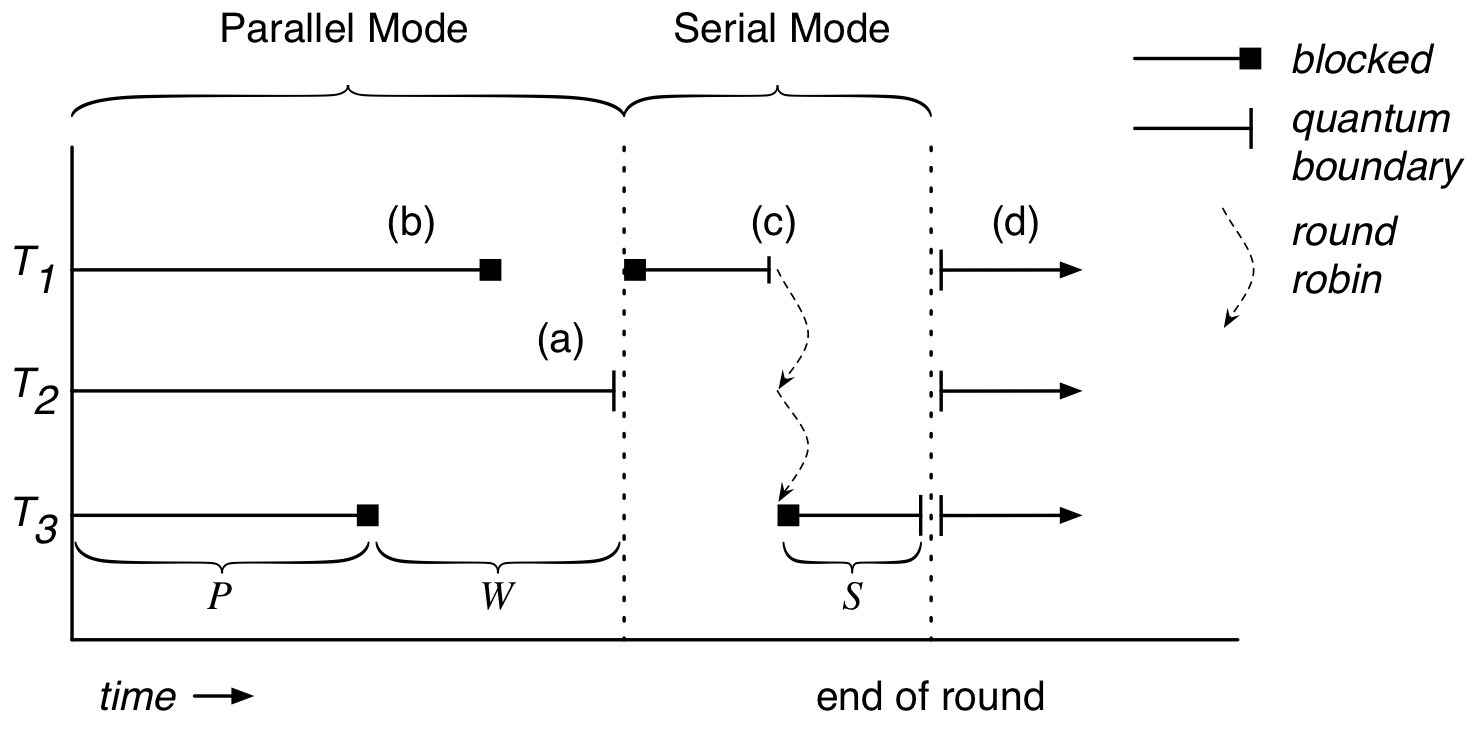
\includegraphics{./figures/quantum.png} }}
  \end{center}
  \caption{Example of a quantum with three threads T1, T2 and T3
    originally from Bergan et al.~\cite{coredet}.  Note that T2 does
    not execute a serial turn because it executed all instructions
    allocated to it for the quantum in parallel mode.}
  \label{fig:quantum}
\end{figure}

Serializing the entire program as described above defeats the
performance advantages of programming using threads.  In their paper,
Devietti et al.\ make the point that if two instructions do not
communicate, the order in which they execute is irrelevant~\cite{dmp}.
Therefore, deterministic execution can be achieved by carefully
controlling only those instructions that cause interthread
communication via shared memory.  By controlling the order in which
load/store instructions to shared memory execute, each dynamic
instance of a load instruction can be made to always read data from
the same dynamic instance of a store instruction.

Using this idea, and keeping the concepts of rounds, quanta and a
deterministic token, parallelism can be recovered by allowing threads
to execute in parallel so long as they do not communicate.  To do
this, each quantum is broken into two modes: \emph{parallel mode} and
\emph{serial mode}.  Figure~\ref{fig:quantum} illustrates three
threads executing a quantum.  In parallel mode, all threads execute
concurrently.  Each thread executes in parallel mode until either:

\begin{itemize}
\item It reaches the end of its quantum.

\item It attempts to access a memory location that may cause
  interthread communication.
\end{itemize}

At the start of each round, all threads execute the parallel segment
of the current quantum and block waiting for serial mode to begin when
one of the above conditions is met.  Serial mode begins after all
threads have finished executing their parallel segment.  Once this
occurs, execution is serialized by passing the deterministic token and
allowing each thread to run their serial segment in isolation.  At
this time, each thread is allowed unrestricted access to shared memory
(both reads and writes).  For each thread, serial mode ends once it
executes the remainder of the instructions in its quantum (which may
be zero, if the first condition marks the end of its parallel
segment).  When a thread finishes executing its serial segment, it
passes the deterministic token to the thread that will execute next
and blocks waiting for serial mode to end.  After all threads finish
executing their serial segments, a new round begins with each thread
executing the parallel segment of the next quantum.

Determinism in DMP is guaranteed on the same input for the following
reasons:

\begin{itemize}
\item No interthread communication can occur during parallel mode as
  it is detected and deferred until serial mode.

\item Each thread's parallel segment will end at a deterministic point
  because, given the same input, a thread will always follow the same
  execution path leading to either the first or second condition being
  met.

\item Serial mode is deterministic because threads are executed
  serially in a deterministic order.
\end{itemize}

In their paper, the deterministic token is passed in thread creation
order from oldest to youngest.  Thread creation and destruction are
deferred until serial mode.  Newly created threads are placed at the
end of the deterministic execution order but do not begin executing
until parallel mode.

All threads in the same process have access to the same shared memory
space.  Therefore, it might seem that any access to shared memory
should be detected as possible interthread communication.  However, in
practice threads often store private data in this same memory space
that is never accessed by other threads.  A thread accessing its own
private data should not have to block for serial mode.  Similarly, it
is common for shared data to be accessed in a read-only manner amongst
several threads.  A thread should not have to block to read shared
read-only data as this cannot cause nondeterminism.

Therefore, in order to accurately detect that interthread
communication is about to occur via a read/write to shared memory, the
ownership/sharing state of each memory location must be tracked.  To
do this, a global \emph{ownership table} is maintained that, for each
memory location, tracks its shared state and, if the memory location
is not shared, its current owner.  The granularity of each entry in
the ownership table can be of any size such as byte-, word- or
page-level.  Choosing a size involves a trade-off between accuracy and
performance.  A memory location can either be shared amongst all
threads or privately owned by a single thread.  Before executing each
load/store instruction to shared memory during parallel mode, the
ownership table is consulted and the instruction is either allowed to
execute or the thread is made to block for serial mode.  An
\emph{ownership table policy} defines the following:

\begin{itemize}
\item When an entry in the ownership table transitions between being
  marked as shared or private.

\item When the ownership of an entry in the ownership table
  transitions from one thread to another.

\item When a thread executing in parallel mode is allowed to proceed
  with a memory access.
\end{itemize}

\begin{table}
  \begin{tabular}{l|l}
    read/write &  parallel mode action              \\
    \hline
    read       &  proceed                           \\
    write      &  block, set private+owned, proceed \\
  \end{tabular}
  \caption{Ownership table policy for shared objects used in DMP paper}
  \label{table:ownership-policy-shared}
\end{table}

\begin{table}
  \begin{tabular}{l|l|l}
    owned & read/write &  parallel mode action           \\
    \hline       
    yes   &  either    &  proceed                        \\
    no    &  read      &  block, set shared, proceed     \\
          &  write     &  block, set priv+owned, proceed \\
  \end{tabular}
  \caption{Ownership table policy for private objects used in DMP paper}
  \label{table:ownership-policy-private}
\end{table}

Table~\ref{table:ownership-policy-shared} and
Table~\ref{table:ownership-policy-private} summarize the ownership
table policy used by DMP~\cite{dmp} when accessing shared objects and
private objects, respectively.  Note that during serial mode, while a
thread does not need to block to access a memory location, the
transitions between shared and private in the table still occur.  The
ownership status of a memory location is only relevant if the memory
location is marked as private in the ownership table.  If a memory
location is private, only the thread marked as its owner is allowed to
access it during parallel mode.  All other threads must block for
serial mode to access that location.  A thread becomes the owner of a
memory location marked as private when it writes to that location in
serial mode after blocking.  This policy ensures that a thread does
not have to block to access its own private data, and also ensures
that changes to private data by its owner are made visible to other
threads at a deterministic point in time, i.e. during serial mode.
Figure~\ref{fig:ownership-graph} shows the possible state transitions
for a memory location accessible by two threads $t$ and $u$.

\begin{figure}[!]
  \begin{center}
    {\resizebox{3.10in}{!}{
        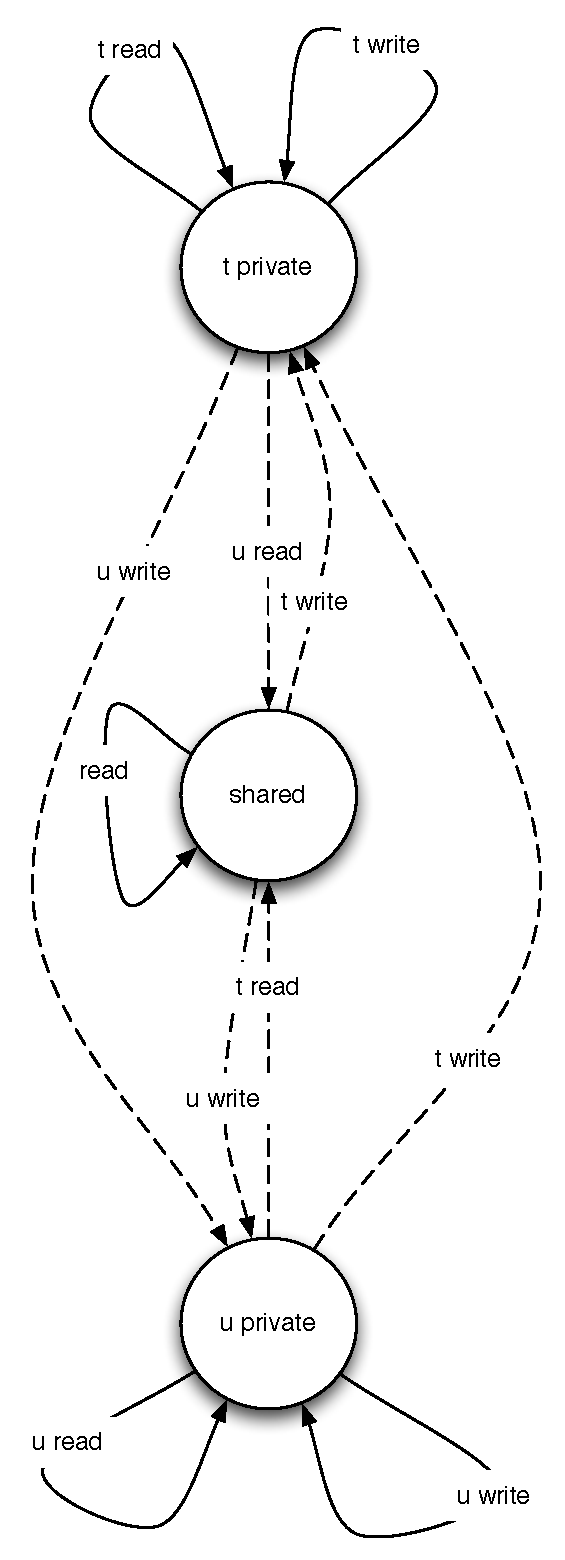
\includegraphics{./figures/ownership-graph.pdf} }}
  \end{center}
  \vspace{-4mm}
  \caption{Ownership transition graph for a memory location accessible to two
    threads.}
  \label{fig:ownership-graph}
\end{figure}

In order to improve the performance of data shared in a read-only
manner, when a memory location marked as private is read by a thread
that is not its owner, that memory location transitions to being
marked as shared.  A memory location marked as shared has no owner.
While it is marked as shared, any thread can read that memory location
during parallel mode without blocking, but writes can only be made in
serial mode.  A memory location marked as shared transitions back to
being marked as private when a thread blocks and writes to it in
serial mode, and in doing so becomes its owner.

During parallel mode, a thread is allowed full access to memory marked
as private that it owns and read-only access to memory marked as
shared.  For all other accesses, a thread must first block for serial
mode.  Note that during parallel mode, the ownership table is strictly
read-only.  A thread is only allowed to modify the ownership table
during serial mode.  No synchronization of the ownership table is
needed during serial mode as only one thread may be executing at a
time.

To see that the above policy makes sense, first consider a policy that
considers the ``owned'' column of Table~\ref{table:ownership-policy}
but ignores the ``shared/private'' and ``read/write'' columns.  Under
such a policy, a thread can access a memory location in parallel mode
only if it is the current owner, therefore ensuring determinism as no
interthread communication can occur.  Next, add the ``shared/private''
and ``read/write'' columns back into the policy.  Now a thread can
access a memory location in parallel mode if it is the current owner
or if it is shared and the access is a read.  This change does not
affect determinism because a shared memory location cannot be written
to by any thread until serial mode, therefore a read access during
parallel mode cannot cause nondeterminism.  Transfer of ownership and
transitions between shared and private are performed after a thread
has blocked for serial mode and are done in an attempt to take
advantage of the principle of locality.  If a thread is likely to
access a memory location again, it is logical to modify the ownership
table such that its next access will not cause it to block.  However,
any policy for modifying the shared/private status of a memory
location during serial mode is acceptable so long as it is
deterministic.

As mentioned previously, quanta can be constructed using any policy so
long as it is deterministic.  In their paper, Devietti et al.\ discuss
several policies for constructing quanta~\cite{dmp}.  They refer to
these as \emph{quantum building policies}.  They experiment with
several different policies:

\begin{itemize}
\item Each quantum lasts until $N$ instructions have been performed.

\item Each quantum lasts until an unlock operation is performed.

\item Each quantum lasts until $N$ consecutive accesses to memory
  marked as private have been performed.

\item Boolean $OR$ of the second and third policies.
\end{itemize}

The first policy is the simplest to implement and simply locks a
quantum down to a fixed size.  The second and third policies try to
detect when a thread has left a critical section, hopefully marking
the end of a period of interthread communication.  In their paper,
Devietti et al.\ also experiment with two styles of serial
mode~\cite{dmp}:

\begin{itemize}
\item Serial mode lasts until the end of the quantum.

\item Serial mode lasts until the end of the quantum or until the
  thread performs an unlock operation and the thread is not holding
  any other locks.
\end{itemize}

They refer to the first style as \emph{full serial mode} and the
second style as \emph{reduced serial mode}.  Reduced serial mode is an
attempt to end serial mode at the end of a critical section in which
interthread communication occurs.  Reduced serial mode greatly
improves the performance of DMP for certain applications, as we will
see in Chapter~\ref{RESULTS}.

For a given round, the ideal quantum building policy would result in
the parallel segments of each thread being precisely the same length
and the serial segments of each thread being zero-length.  A quantum
in which each parallel segment is precisely the same length is called
\emph{balanced} and is ideal because it minimizes the amount of time
each thread blocks waiting for serial mode.  A quantum with a
zero-length serial mode is ideal because it minimizes serialization.
In practice, most programs will not have a zero-length serial mode as
there will be a varying amount of interthread communication.
Therefore, the question of how long serial mode should be comes into
question.  If serial mode is too short, a thread with many consecutive
shared memory accesses may not be able to complete them all in its
serial segment and may block too soon into its next parallel segment,
likely leading to imbalance.  If serial mode is too long, parallelism
is reduced by making the execution too serialized.

Devietti et al.\ argue that deterministic execution should be used not
only for debugging but should be left on when the product is deployed.
Their paper advocates for a change in multiprocessor system
architecture such that deterministic execution using the methods
described are implemented in hardware.  In their implementation, they
use the cache line state maintained by the MESI cache coherence
protocol (MESI stands for Modified, Exclusive, Shared and Invalid, the
four states in the protocol's state diagram) to track ownership
status.  To evaluate their ideas, they simulate a hardware
implementation of DMP using Pin, a program analysis tool.

There are both advantages and disadvantages to the DMP method of
deterministic execution.  DMP makes no assumptions about the behavior
of the program.  Other frameworks require a program be data-race free
in order to guarantee determinism.  However, it is important to note
that DMP will always execute a program such that communicating
instructions are interleaved in the same order.  DMP does not control
non-communicating instructions, which may be interleaved or may occur
simultaneously in any order.  Two executions in which all
communicating instructions are ordered the same are known as
\emph{communication-equivalent interleavings}.

If the particular set of communication-equivalent interleavings that
DMP generates reveals a bug for a given input, that bug will occur
every time the program is executed with that same input.  DMP is not a
tool for automatically uncovering concurrency bugs.  However, running
a program with DMP makes it easy to fix concurrency bugs that surface
when the program is run with a given input.  However, testing a
program with DMP can only guarantee that the program is bug-free when
run using that input and when run using the thread interleavings
generated by DMP.  It is possible that other bugs exist but do not
surface with the particular set of interleavings DMP allows.  This is
a definite disadvantage of DMP.  If the overhead of leaving DMP on
when deploying a product is too large, a product might be extensively
tested with DMP across a wide range of inputs, but miss bugs that only
surface after the product is deployed with DMP turned off.  Therefore,
to be most effective the overhead of DMP must be small enough that it
can be left on across the life of the product.

Their experimental results show that deterministic execution can be
achieved with acceptable performance using DMP implemented in
hardware.  Hardware DMP using an ownership table incurred a slowdown
of between 37\% and 15\%.

\section{CoreDet}

CoreDet is an implementation of DMP in software.  Bergan et al.\ use a
modified LLVM (Low Level Virtual Machine) C/C++ compiler with several
new compiler phases that add instrumentation code before load and
store instructions to shared memory~\cite{coredet}.  The
instrumentation code calls into the CoreDet run-time framework that
consults an in-memory ownership table and decides if the instruction
can be executed immediately or must wait for serial mode.  The
ownership table and all other data structures needed by the framework
are stored in global shared memory.  A major contribution of CoreDet
is that it shows that DMP can be implemented effectively in software
and it extends the original DMP paper by adding two new approaches to
deterministic execution.

The first approach drops the use of a global ownership table to
prevent uncontrolled interthread communication.  Instead, each thread
has a local store buffer that caches writes to shared memory made
during parallel mode.  When a thread reads a location, it first
consults its store to see if it has a modified value for that location
and otherwise retrieves the value from global shared memory.  This
means that shared memory is read-only during parallel mode.  Writes
cached in a thread's store buffer are committed to global shared
memory in a new commit mode that occurs between parallel mode and
serial mode.  A clever algorithm allows most commits to be made in
parallel while still preserving the deterministic commit order.  This
is done by allowing threads to commit in parallel while maintaining
enough metadata to prevent one thread's writes from overwriting some
other thread that comes after it in the deterministic commit order.
By using a store buffer, the need to block for serial mode is greatly
reduced.  Parallel mode ends when either of the following conditions
hold:

\begin{itemize}
\item A memory fence instruction is reached.

\item An atomic operation such as a compare-and-swap must be
  performed.
\end{itemize}

The second approach combines ownership tracking with the store buffer.
The global ownership table is brought back and is maintained as it was
in the original DMP paper, thus allowing distinction of accesses to
shared data from accesses to private data.  While in parallel mode, a
thread can access its own private data without blocking and without
consulting its local store, but accesses to another thread's private
data must wait until serial mode.  If a thread wishes to access shared
data while in parallel mode, it must consult its local store.  This
second approach reduces the overhead incurred by the frequent
consulting of the store buffer that the original approach suffers
from.

For their evaluation, they implement three versions of DMP: one using
the ownership table introduced in the original DMP paper, a second
using a store buffer and a third using a combination of both.  Their
results show that the ownership table has low overhead but limited
scalability as execution becomes more serialized as the number of
threads is increased.  The store buffer implementation offers good
scalability but higher overhead due to the high cost required to
access and maintain the store buffer.  The performance of using both
the ownership table and a store buffer is somewhere in between the
first two in terms of scalability and overhead.

\section{Kendo}

Kendo is a software framework that offers a weak determinism guarantee
for lock-based, data-race free C/C++ code.  Olszewski, Ansel, and
Amarasinghe guarantee determinism using Kendo for data-race free
programs by guaranteeing a deterministic order of all lock
acquisitions for a given program input~\cite{kendo}.  Kendo implements
a subset of the POSIX Threads API, replacing the existing
synchronization functions (such as $pthread\_mutex\_lock$,
$pthread\_mutex\_unlock$, etc.) with calls to their own run-time
framework.  Programs run using Kendo must first be recompiled and
linked with the Kendo run-time framework.

In order to achieve its goal of weak determinism, each thread
maintains a \emph{deterministic logical clock} that is incremented
deterministically, potentially after every instruction.  Each lock
stores the deterministic logical clock of the last thread to release
the lock.  In their basic algorithm, a thread attempting to acquire
the lock must wait until all threads with smaller thread ID's have
greater deterministic logical clock and all threads with larger thread
ID's have greater or equal deterministic logical clocks.  Using these
rules, Kendo maintains the invariant that only one thread may hold a
lock at a given logical time in order to guarantee determinism.

Kendo is an effective and fairly lightweight method of guaranteeing
deterministic execution, however in order to guarantee determinism it
requires that a program be data-race free.  A program will not execute
deterministically using Kendo unless all shared data is protected by a
consistent set of locks.  This hurts its usefulness, especially in
debugging parallel programs, as having a deterministic guarantee while
trying to debug a multithreaded program is one of the main goals of
deterministic execution.

\section{Grace}

Grace is a run-time framework that enables safe and efficient
concurrent programming.  Programs executed using Grace are said to be
\emph{behaviorally equivalent} to their sequential counterparts.  This
means a program executed using Grace will produce the same output as
the original program executed with thread spawns converted to regular
function invocations.  The order in which functions would be invoked
in this single-threaded version is known as \emph{program order}.
Grace is designed for fork-join parallelism applications in which a
parent function spawns one or more children and then waits for them to
terminate before returning itself.  Berger et al.\ designed Grace in
an attempt to get rid of a large number of concurrency bugs while
still achieving good performance~\cite{grace}.  The concurrency bugs
that Grace eliminates and their causes are:

\begin{itemize}
\item Deadlocks - cyclic lock acquisition.

\item Race conditions - unguarded updates.

\item Atomicity violations - unguarded, interleaved updates.

\item Order violations - threads scheduled in unexpected order.
\end{itemize}

Grace achieves its goal by allowing multiple threads to execute
simultaneously, but executes each thread in a separate transaction
such that they are isolated and appear to execute atomically.  Grace
prevents a thread from committing its transaction to shared memory
until all of its logical predecessors have committed successfully.  In
the case of a parent spawning one or more children, this means a
parent cannot commit until all of its children have committed.  In the
case of a child thread, this means it cannot commit until all of its
siblings who were spawned earlier by its parent have committed.  Grace
eliminates the above sources of concurrency bugs in the following
manner:

\begin{itemize}
\item No deadlocks - all lock acquisitions/releases are converted to
  no-ops.

\item No race conditions - all transactions commit changes to shared
  memory in a deterministic order.

\item No atomicity violations - all threads execute atomically in an
  isolated transaction.

\item No order violations - threads are executed in program order.
\end{itemize}

Grace uses virtual memory-based software transactional memory to allow
concurrent execution of multiple threads while still ensuring that
execution is behaviorally equivalent to a serial execution.  To do
this, each memory location stores a version number that is incremented
whenever it is updated.  Using the operating system's virtual memory
facilities, each thread is given two mappings of shared memory: a
shared mapping that reflects the last successful commit and a private
copy-on-write mapping used for local changes.  As a thread executes,
it maintains a read-set and write-set containing the memory locations
that it read from and wrote to, respectively.  When a thread is ready
to terminate, it must commit all changes in its write-set to shared
memory.  To do this, it checks the committed versions numbers to those
in its read set.  If they match, the commit is allowed.  Otherwise,
the thread aborts as its calculations were performed on out-of-date
data.  The thread must abort and be re-executed using the new memory
space.

Because threads commit in program order, Grace is designed for
applications with many small, short-running threads such that threads
do not wait very long before they can commit. Because Grace runs
threads in isolation using transactions, Grace is restricted to a
subset of parallel applications.  For instance, Berger et
al.~\cite{grace} note that the following thread behaviors are not
supported:

\begin{itemize}
\item Threads that run infinitely or until program is terminated.

\item Threads that perform interthread communications (i.e., via
  synchronization primitives such as condition variables).
\end{itemize}

This means that Grace cannot work as a general solution to
deterministic execution.

\section{Deterministic Parallel Java}

Deterministic Parallel Java (DPJ) is an extension to the Java
programming language that adds parallel code blocks as well as a
\emph{type and effect} system that allows a compile-time guarantee of
determinism~\cite{dpj}.  DPJ splits the heap into named
\emph{regions}.  DPJ source code is annotated to indicate in which
region a data member is allocated.  Similarly, method definitions are
annotated to indicate which regions they read and which regions they
write (known as \emph{read effects} and \emph{write effects}).  The
region into which each object is allocated is computed at
compile-time.  Using the annotations provided by the programmer in the
source code, the DPJ compiler determines if a given program will
execute deterministically.  This is done by ensuring that all pairs of
memory accesses are either both reads, access disjoint regions of the
heap or are properly synchronized to prevent concurrent access.

DPJ uses compile-time enforcement of determinism, meaning its overhead
at run-time is very small when compared to other solutions such as
DMP.  However, it could be argued that the type and effect systems
used by DPJ is clumsy and frustrating to the programmer.  The
annotations that must be provided by the programmer can wind up being
very complicated and hard to understand.  Furthermore, determinism can
only be guaranteed if every annotation is correct, and the burden to
fix any inaccuracies is placed on the programmer.

\section{maTe DMP}

My thesis is that a Java-like programming language can be executed
deterministically using DMP with less overhead than a C-like
programming language.  A Java-like language is object-oriented where
objects are accessed through references, is byte-compiled and is
executed in a virtual machine.  A C-like language contains primitive
data-types, pointers and is compiled to native code.  In my research,
I modified maTe, a Java-like language, and used it to test my thesis.
I built upon existing work in the area of deterministic execution to
implement DMP inside the maTe virtual machine using quanta and an
ownership tracking system.

As described earlier, DMP relies on an ownership tracking mechanism to
maintain the shared/private status of each memory location in shared
memory in order to detect interthread communication that can cause
nondeterminism.  When detected, execution of each thread is serialized
for a small period of time so that communication is performed in a
deterministic order.  The ownership table policy determines how memory
locations transition between shared/private during serial mode.  This
policy is important not only because it is used to enforce determinism
but also because it has a large effect on performance.  For example, a
policy that relies only on thread ownership will yield worse
performance than a policy that also takes into account private/shared
status and whether the access is a read or write.

The key idea of my thesis is that, in a Java-like language where
shared memory can only be accessed through object references, the
ability of a thread to access a memory location can be determined at
any point by traversing the global object graph.  Compare this to
C-like languages where, through the use of pointers, arbitrary memory
locations can be accessed and no memory location can be truly
considered private.  While escape analysis at compile-time can
determine that an object is thread local, it cannot prevent the use of
unsafe memory operations at run-time.  Therefore any ownership
tracking technique used in such a language must be conservative.

Executing inside of a virtual machine also offers advantages to
deterministic execution.  In the Java virtual machine, each method
frame has its own local variable array and operand stack that are
private and cannot be accessed by other threads (or even other methods
executing in the same thread).  Therefore, instructions that operate
on these locations need not be instrumented, reducing overhead.  The
same cannot be said of C, in which a thread's stack is located in
shared memory space.

\begin{figure}[!]
  \begin{center}
    {\resizebox{\textwidth}{!}{
        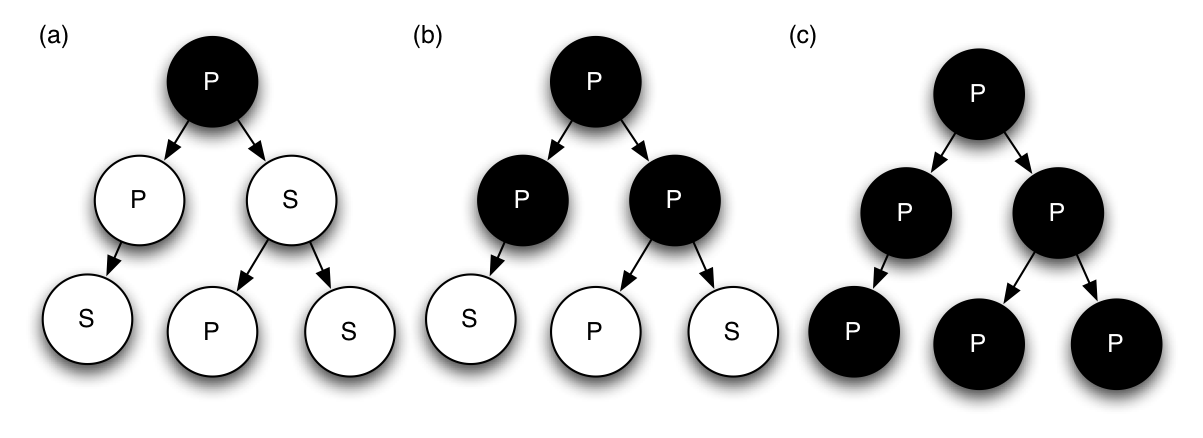
\includegraphics{./figures/depth.png} }}
  \end{center}
  \caption{Example of changes in ownership due to a write using depth 1 (a), 2
    (b) and 3 (c).}
  \label{fig:depth}
\end{figure}

As mentioned earlier, large chunks of memory can be privatized quickly
by choosing a large granularity for the ownership table.  This is done
in the hope of avoiding the need to block to access nearby memory in
the future.  In a C-like language, two memory locations are ``nearby''
if their addresses in memory are nearby.  ``Nearby'' has a different
meaning in a Java-like language as there is no concept of addresses.
Instead, the relative distance between two objects is computed by
finding the shortest path between them in the global object graph.
Therefore, in my implementation, the granularity of the ownership
table is given not in units of bytes, words or pages but in depth.  At
a depth of one, only the ownership table entry of the object being
accessed is modified, at a depth of two, the object being modified as
well as all objects it references are modified and so on.
Figure~\ref{fig:depth} illustrates the changes in object ownership
that occur when writing to the object at the root of the tree using an
ownership table depth of 1, 2 and 3.  Blackened objects are those
marked as private and owned by the writing thread.

In order to test my thesis, I extended the maTe programming language
and implemented DMP using an ownership table in the maTe virtual
machine.  I did not implement the local store buffer used by
CoreDet~\cite{coredet}, however I did implement the option to run
using \emph{reduced serial mode}.  maTe is a pure object-oriented,
byte-compiled, garbage-collected programming language.  maTe features
support for single inheritance, virtual method calls, method and
operator overloading, nested local variable declarations and basic
input/output facilities.  maTe includes no primitive data types.
Instead, maTe includes four predefined classes to allow for integer
arithmetic, text manipulation and simple data storage: Object,
Integer, String and Table (Table is a key/value pair hash map inspired
by Java's $java.util.HashMap$ class).

Grammatically, maTe source is very similar to Java source code.  An
example of maTe source code can be seen in Figure~\ref{fig:mate-code}.
maTe source code is translated by the maTe compiler to an intermediate
maTe assembly language before being assembled by the maTe assembler
into a platform independent binary class file.  Class files are
executed inside the maTe virtual machine, which implements the maTe
instruction set as well as the predefined classes in native code.

\begin{figure}[!]
\begin{small}
  \small \bnncode
  \codeln. class Point \{ \\
  \codeln. \> Integer x, y; \\
  \codeln. \> Point(Integer x, Integer y) \{ this.x = x; this.y = y; \} \\
  \codeln. \> Point operator+(Point p) \{ return new Point(x + p.x, y + p.y); \} \\
  \codeln. \> Integer equals(Object obj) \{ \\
  \codeln. \>\> if (obj == null) return 0; \\
  \codeln. \>\> if (obj instanceof Point) \{ \\
  \codeln. \>\>\> Point p; \\
  \codeln. \>\>\> p = (Point)obj; \\
  \codeln. \>\>\> if (x.equals(p.x) \&\& y.equals(p.y)) \{ \\
  \codeln. \>\>\>\> return 1; \\
  \codeln. \>\>\> \} \\
  \codeln. \>\> \} \\
  \codeln. \>\> return 0; \\
  \codeln. \> \} \\
  \codeln. \> String toString() \{ return "(" + x.toString() + ", " + y.toString() + ")"; \} \\
  \codeln.  \} \\
  \codeln. Integer main() \{ \\
  \codeln. \> Point p, q, r; \\
  \codeln. \> p = new Point(10, 10); \\
  \codeln. \> q = new Point(5, 5); \\
  \codeln. \> r = p + q; \\
  \codeln. \> out "p = " + p.toString() + newline; \\
  \codeln. \> out "q = " + q.toString() + newline; \\
  \codeln. \> out "r = " + r.toString() + newline; \\
  \codeln. \> return 0; \\
  \codeln. \}
  \ecode \vspace{-0mm}
  \caption{\label{fig:mate-code} Example of maTe source code.}
\end{small}
\end{figure}

Architecturally, the maTe virtual machine is modeled after the Java
virtual machine.  Method frames are stored on a global stack with each
method frame holding a local variable array and operand stack.  The
local variable array stores arguments and local variables.  The
operand stack stores parameters to be passed to methods and receives
method results.  Upon startup, the class file to be executed is loaded
into memory and an in-memory version of the class table is generated.
Memory for new objects is allocated from a global heap.  The maTe
instruction set is also modeled after Java.  It uses high level
instructions that allows implementation of much of the method
dispatch/stack maintenance to be pushed up to the virtual machine
instead of being handled by the compiler.

The current implementation of the maTe language is done in a mix of C
and C++.  The assembler and virtual machine are implemented in C while
the compiler is written in C++ using flex/bison as the scanner/parser
generator.  The maTe virtual machine includes a conservative
concurrent, snapshot-at-the-beginning garbage collector implemented
using the tri-color abstraction and a mark stack.  The garbage
collector is run in a separate thread using the $pthreads$ threading
library.

%%% Local Variables: 
%%% mode: latex
%%% TeX-master: "thesis"
%%% End: 
